\documentclass[11pt]{article}

\usepackage[margin=1in]{geometry}
\usepackage{amsmath, amssymb}
\usepackage{graphicx}
\usepackage{booktabs}
\usepackage{hyperref}
\usepackage{xcolor}
\usepackage{enumitem}

\hypersetup{
    colorlinks=true,
    linkcolor=blue,
    urlcolor=blue,
    citecolor=blue
}

\title{Modified PIANO: A Physics-Informed DeepONet Framework \\ for Satellite-Based Precipitation Nowcasting}
\author{}
\date{}

\begin{document}

\maketitle

\section{Overview}

This methodology extends the original PIANO framework by replacing its CNN-based temporal neural operator (T-NO) with a \textbf{physics-informed DeepONet (PI-DeepONet)}. The velocity-estimation stage (V-NO) is kept unchanged. The goal of the modification is to move from a fixed-grid, fixed-horizon image-to-image predictor to a \textbf{continuous, resolution-independent, mesh-free operator} that can be queried at arbitrary spatial locations and lead times, while remaining physically consistent with an advection process.

The framework still factorizes the nowcasting problem into two sub-tasks:

\begin{enumerate}
    \item \textbf{Velocity estimation} --- infer the motion field driving the evolution of the precipitation/cloud field from satellite imagery.
    \item \textbf{Temporal propagation} --- advance the current atmospheric state forward in time using that velocity field.
\end{enumerate}

Only sub-task 2 changes. Figure~\ref{fig:architecture} illustrates the full modified pipeline.

\begin{figure}[htbp]
    \centering
    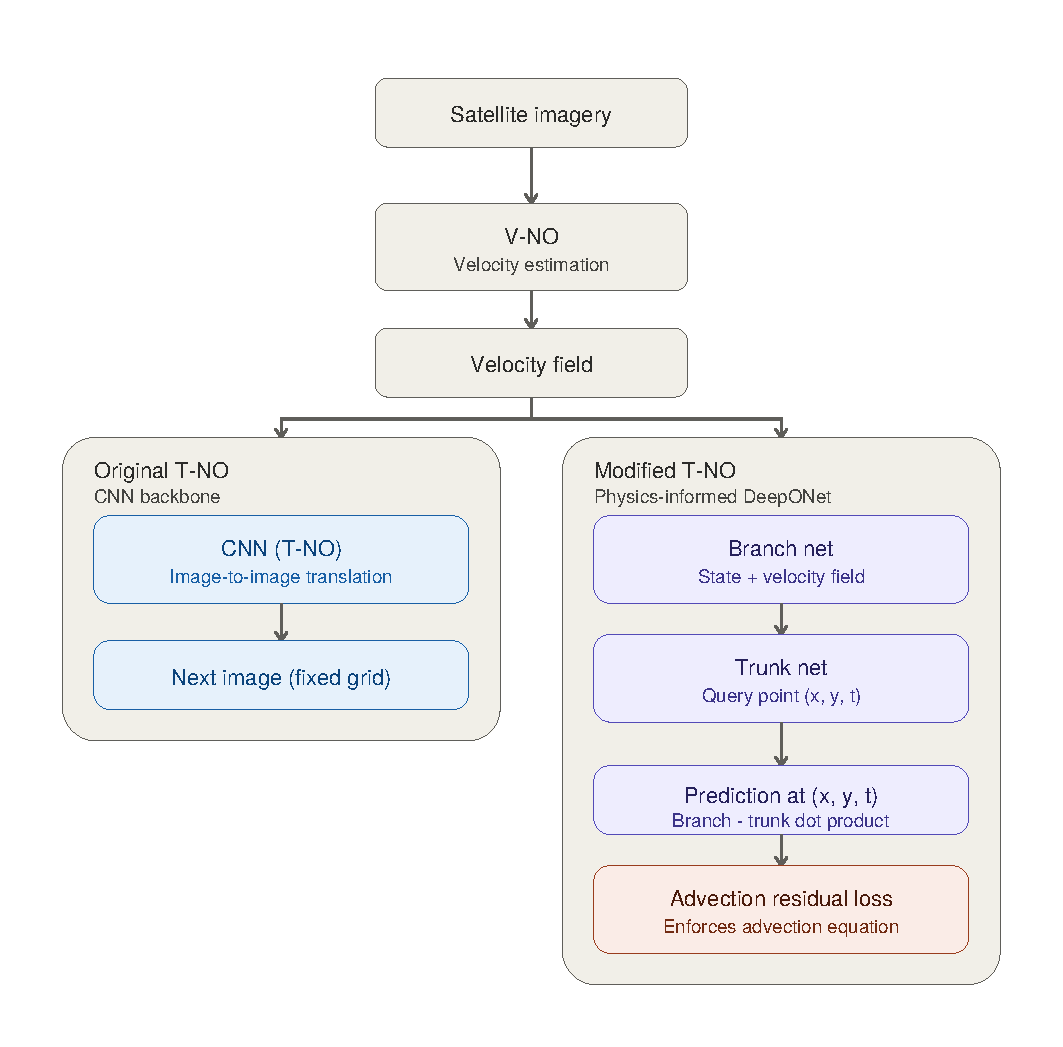
\includegraphics[width=0.72\textwidth]{piano_diagram.pdf}
    \caption{Modified PIANO architecture. The shared V-NO stage (top) is unchanged. The original CNN-based T-NO (left) maps directly to a fixed-grid next image. The proposed T-NO (right) is a physics-informed DeepONet, in which a branch net encodes the current state and velocity field, a trunk net encodes an arbitrary space-time query coordinate $(x,y,t)$, and their combination is regularized by an advection-residual physics loss.}
    \label{fig:architecture}
\end{figure}

\section{Problem Formulation}

Let:
\begin{itemize}
    \item $I(x, y, t_0) \in \mathbb{R}^{H \times W \times C}$ be the satellite image stack (e.g.\ IR/WV channels) at the current time $t_0$, over a spatial grid $(x, y) \in \Omega \subset \mathbb{R}^2$.
    \item $\mathbf{v}(x, y) = (u(x,y), w(x,y))$ be the 2D velocity (motion) field estimated from the imagery.
    \item $s(x, y, t)$ be the scalar precipitation/brightness-temperature field we want to predict at future time $t = t_0 + \Delta t$.
\end{itemize}

The task is to learn an operator

\begin{equation}
\mathcal{G}: \big(I(\cdot, \cdot, t_0), \mathbf{v}(\cdot,\cdot)\big) \;\longmapsto\; s(x, y, t)
\end{equation}

that can be evaluated at \textbf{any} query coordinate $(x, y, t)$, not just the coordinates present in the training grid.

\section{Stage 1 --- V-NO (Unchanged)}

The V-NO remains a convolutional encoder that maps a short sequence of past satellite frames to a dense velocity field:

\begin{equation}
\mathbf{v}(x, y) = \text{V-NO}\big(I(\cdot,\cdot,t_{-k}), \dots, I(\cdot,\cdot,t_0)\big)
\end{equation}

Implementation, loss, and training schedule for V-NO are retained from the original PIANO paper (no change proposed here).

\section{Stage 2 --- T-NO as a Physics-Informed DeepONet}

\subsection{Architecture}

The modified T-NO follows the standard DeepONet decomposition into a \textbf{branch net} and a \textbf{trunk net}, whose outputs are combined via an inner product.

\paragraph{Branch net $\mathcal{B}_\theta$}
\begin{itemize}
    \item Input: the current state $I(\cdot,\cdot,t_0)$ and velocity field $\mathbf{v}(\cdot,\cdot)$, both sampled at a fixed set of $m$ sensor locations on $\Omega$.
    \item A CNN encoder (e.g.\ a small ResNet stem) first compresses the raw image and velocity channels into a feature map, which is flattened and passed through fully connected layers.
    \item Output: a latent coefficient vector $\mathbf{b} \in \mathbb{R}^p$.
\end{itemize}

\begin{equation}
\mathbf{b} = \mathcal{B}_\theta\big(I(\cdot,\cdot,t_0), \mathbf{v}(\cdot,\cdot)\big)
\end{equation}

\paragraph{Trunk net $\mathcal{T}_\phi$}
\begin{itemize}
    \item Input: a query coordinate $(x, y, t)$ --- any spatial location and any future lead time, not restricted to the training grid.
    \item A small MLP (with sinusoidal/Fourier positional encoding of $(x,y,t)$ recommended, to help the network represent high-frequency spatial detail).
    \item Output: a latent basis vector $\boldsymbol{\tau} \in \mathbb{R}^p$.
\end{itemize}

\begin{equation}
\boldsymbol{\tau} = \mathcal{T}_\phi(x, y, t)
\end{equation}

\paragraph{Combination (prediction)}

\begin{equation}
\hat{s}(x, y, t) = \sum_{k=1}^{p} b_k \, \tau_k \;+\; b_0
\end{equation}

where $b_0$ is a bias term (standard DeepONet practice).

\subsection{Why This Preserves PIANO's Conceptual Split}

\begin{itemize}
    \item The branch net still plays the role of ``what is the current situation'' (state + velocity), matching T-NO's original input.
    \item The trunk net replaces the fixed output grid with a continuous query mechanism --- the model is now a function of $(x,y,t)$ rather than a fixed-size decoder.
\end{itemize}

\section{Physics-Informed Loss}

\subsection{Data (Reconstruction) Loss}

Standard supervised term against ground-truth satellite/precipitation fields at the sampled training query points:

\begin{equation}
\mathcal{L}_{\text{data}} = \frac{1}{N} \sum_{i=1}^{N} \big(\hat{s}(x_i, y_i, t_i) - s^{\text{true}}(x_i, y_i, t_i)\big)^2
\end{equation}

\subsection{Physics (Advection Residual) Loss}

The governing assumption is that the field is transported by the estimated velocity field, i.e.\ it approximately satisfies the advection equation:

\begin{equation}
\frac{\partial s}{\partial t} + u(x,y)\frac{\partial s}{\partial x} + w(x,y)\frac{\partial s}{\partial y} = 0
\end{equation}

Because $\hat{s}(x,y,t)$ is produced by a DeepONet with a differentiable trunk net, the required partial derivatives $\partial \hat{s}/\partial t$, $\partial \hat{s}/\partial x$, $\partial \hat{s}/\partial y$ can be obtained by automatic differentiation with respect to the trunk net's input coordinates --- exactly as in the physics-informed DeepONet formulation used for PDE operator learning.

The residual is evaluated at a set of $N_r$ collocation points $(x_j, y_j, t_j)$ sampled densely (and randomly) in space-time, not just at labeled data points:

\begin{equation}
\mathcal{L}_{\text{phys}} = \frac{1}{N_r} \sum_{j=1}^{N_r} \left( \frac{\partial \hat{s}}{\partial t}\Big|_j + u_j \frac{\partial \hat{s}}{\partial x}\Big|_j + w_j \frac{\partial \hat{s}}{\partial y}\Big|_j \right)^2
\end{equation}

\subsection{Combined Objective}

\begin{equation}
\mathcal{L}_{\text{total}} = (1-\alpha)\, \mathcal{L}_{\text{data}} + \alpha\, \mathcal{L}_{\text{phys}}
\end{equation}

$\alpha \in [0,1]$ is the physics-weighting hyperparameter, consistent with PIANO's original sensitivity-analysis variable, and should be tuned the same way (sweep and select based on validation CSI/MSE).

\emph{Optional}, following the physics-informed DeepONet paper's practice: add a boundary/initial-condition loss term $\mathcal{L}_{\text{ic}}$ enforcing $\hat{s}(x,y,t_0) = I(x,y,t_0)$, to anchor the operator to the known initial state.

\begin{equation}
\mathcal{L}_{\text{total}} = (1-\alpha)\,\mathcal{L}_{\text{data}} + \alpha\,\mathcal{L}_{\text{phys}} + \lambda_{\text{ic}}\,\mathcal{L}_{\text{ic}}
\end{equation}

\section{Training Procedure}

\begin{enumerate}
    \item \textbf{Pretrain / freeze V-NO} (or train jointly --- follow original PIANO's chosen strategy) to obtain $\mathbf{v}(x,y)$ for each training sample.
    \item \textbf{Sample sensor points} for the branch net input (fixed sensor grid, e.g.\ a downsampled version of $\Omega$).
    \item \textbf{Sample query points} for the trunk net:
    \begin{itemize}
        \item Labeled points $(x_i,y_i,t_i)$ at available ground-truth lead times (1h--8h, matching PIANO's evaluation horizons) for $\mathcal{L}_{\text{data}}$.
        \item Random collocation points $(x_j,y_j,t_j)$ spanning continuous space-time (including non-integer lead times) for $\mathcal{L}_{\text{phys}}$.
    \end{itemize}
    \item \textbf{Forward pass}: compute $\mathbf{b}$ once per sample from the branch net; evaluate the trunk net at all sampled query points; combine to get predictions.
    \item \textbf{Backward pass}: compute $\mathcal{L}_{\text{data}}$, $\mathcal{L}_{\text{phys}}$ (via autodiff through the trunk net w.r.t.\ $x,y,t$), and optionally $\mathcal{L}_{\text{ic}}$; backpropagate the weighted sum $\mathcal{L}_{\text{total}}$.
    \item \textbf{Optimizer}: Adam with learning-rate warmup/decay, consistent with standard DeepONet training recipes; gradient clipping recommended since second-order-adjacent derivative terms can be noisy early in training.
    \item \textbf{$\alpha$ scheduling} (optional improvement over a fixed $\alpha$): start with a low $\alpha$ (data-dominated) and anneal upward, so the network first learns a reasonable fit before being constrained by the physics residual --- mirrors curriculum strategies used in PINN training.
\end{enumerate}

\section{Inference}

At inference time, given a new satellite sequence:

\begin{enumerate}
    \item Run V-NO to obtain $\mathbf{v}(x,y)$.
    \item Run the branch net once to obtain $\mathbf{b}$.
    \item Query the trunk net at \textbf{any} desired $(x,y,t)$ --- arbitrary lead time (not restricted to 1h/2h/.../8h bins), arbitrary spatial resolution, or a cropped region of interest --- without retraining or re-running the branch net.
\end{enumerate}

This is the key practical advantage over the CNN T-NO: one branch-net forward pass amortizes across unlimited query resolutions/horizons.

\section{Evaluation}

Retain PIANO's original evaluation protocol for direct comparability:

\begin{itemize}
    \item \textbf{Critical Success Index (CSI)} at each lead time (1h--8h), computed by querying the trunk net at the corresponding integer-hour coordinates and rasterizing to the original grid for scoring against ground truth.
    \item \textbf{MSE} across lead times.
    \item \textbf{$\alpha$ sensitivity analysis}, replicated for the new formulation, to check whether the optimal physics weight shifts once the operator is coordinate-based rather than grid-based.
    \item \textbf{New metric enabled by this architecture}: prediction consistency across non-integer lead times (e.g.\ 2.5h) and across resolutions, to quantify the resolution-independence benefit --- something the CNN baseline cannot produce natively.
    \item \textbf{Baselines}: compare against the original CNN-based PIANO, plus NPM and PhyDNet, as in the original paper.
\end{itemize}

\section{Summary of Changes vs.\ Original PIANO}

\begin{table}[htbp]
\centering
\begin{tabular}{@{}p{3.1cm}p{4.6cm}p{5.8cm}@{}}
\toprule
\textbf{Component} & \textbf{Original PIANO} & \textbf{Modified PIANO} \\
\midrule
V-NO & CNN velocity encoder & Unchanged \\
T-NO & CNN image-to-image (ResNet/pix2pix-style) & Physics-informed DeepONet (branch + trunk) \\
Output & Fixed-grid image per lead-time bin & Continuous function of $(x,y,t)$ \\
Physics constraint & $\alpha$-weighted advection loss on grid outputs & $\alpha$-weighted advection residual via autodiff on trunk-net coordinates \\
Query flexibility & Fixed resolution, fixed lead-time bins & Arbitrary resolution, arbitrary lead time \\
Added cost & --- & Trunk-net autodiff overhead; collocation-point sampling \\
\bottomrule
\end{tabular}
\caption{Summary of architectural and training differences between the original and modified PIANO frameworks.}
\end{table}

\end{document}
